\documentclass{ximera}

%\usepackage{todonotes}

\newcommand{\todo}{}

\usepackage{esint} % for \oiint
\ifxake%%https://math.meta.stackexchange.com/questions/9973/how-do-you-render-a-closed-surface-double-integral
\renewcommand{\oiint}{{\large\bigcirc}\kern-1.56em\iint}
\fi


\graphicspath{
  {./}
  {ximeraTutorial/}
  {basicPhilosophy/}
  {functionsOfSeveralVariables/}
  {normalVectors/}
  {lagrangeMultipliers/}
  {vectorFields/}
  {greensTheorem/}
  {shapeOfThingsToCome/}
  {dotProducts/}
  {partialDerivativesAndTheGradientVector/}
  {../productAndQuotientRules/exercises/}
  {../normalVectors/exercisesParametricPlots/}
  {../continuityOfFunctionsOfSeveralVariables/exercises/}
  {../partialDerivativesAndTheGradientVector/exercises/}
  {../directionalDerivativeAndChainRule/exercises/}
  {../commonCoordinates/exercisesCylindricalCoordinates/}
  {../commonCoordinates/exercisesSphericalCoordinates/}
  {../greensTheorem/exercisesCurlAndLineIntegrals/}
  {../greensTheorem/exercisesDivergenceAndLineIntegrals/}
  {../shapeOfThingsToCome/exercisesDivergenceTheorem/}
  {../greensTheorem/}
  {../shapeOfThingsToCome/}
  {../separableDifferentialEquations/exercises/}
}

\newcommand{\mooculus}{\textsf{\textbf{MOOC}\textnormal{\textsf{ULUS}}}}

\usepackage{tkz-euclide}\usepackage{tikz}
\usepackage{tikz-cd}
\usetikzlibrary{arrows}
\tikzset{>=stealth,commutative diagrams/.cd,
  arrow style=tikz,diagrams={>=stealth}} %% cool arrow head
\tikzset{shorten <>/.style={ shorten >=#1, shorten <=#1 } } %% allows shorter vectors

\usetikzlibrary{backgrounds} %% for boxes around graphs
\usetikzlibrary{shapes,positioning}  %% Clouds and stars
\usetikzlibrary{matrix} %% for matrix
\usepackage{pgfplots}
\usepgfplotslibrary{polar} %% for polar plots
\usepgfplotslibrary{fillbetween} %% to shade area between curves in TikZ
\usetkzobj{all}
\usepackage[makeroom]{cancel} %% for strike outs
%\usepackage{mathtools} %% for pretty underbrace % Breaks Ximera
%\usepackage{multicol}
\usepackage{pgffor} %% required for integral for loops



%% http://tex.stackexchange.com/questions/66490/drawing-a-tikz-arc-specifying-the-center
%% Draws beach ball
\tikzset{pics/carc/.style args={#1:#2:#3}{code={\draw[pic actions] (#1:#3) arc(#1:#2:#3);}}}



\usepackage{array}
\setlength{\extrarowheight}{+.1cm}
\newdimen\digitwidth
\settowidth\digitwidth{9}
\def\divrule#1#2{
\noalign{\moveright#1\digitwidth
\vbox{\hrule width#2\digitwidth}}}





\newcommand{\RR}{\mathbb R}
\newcommand{\R}{\mathbb R}
\newcommand{\N}{\mathbb N}
\newcommand{\Z}{\mathbb Z}

\newcommand{\sagemath}{\textsf{SageMath}}


%\renewcommand{\d}{\,d\!}
\renewcommand{\d}{\mathop{}\!d}
\newcommand{\dd}[2][]{\frac{\d #1}{\d #2}}
\newcommand{\pp}[2][]{\frac{\partial #1}{\partial #2}}
\renewcommand{\l}{\ell}
\newcommand{\ddx}{\frac{d}{\d x}}

\newcommand{\zeroOverZero}{\ensuremath{\boldsymbol{\tfrac{0}{0}}}}
\newcommand{\inftyOverInfty}{\ensuremath{\boldsymbol{\tfrac{\infty}{\infty}}}}
\newcommand{\zeroOverInfty}{\ensuremath{\boldsymbol{\tfrac{0}{\infty}}}}
\newcommand{\zeroTimesInfty}{\ensuremath{\small\boldsymbol{0\cdot \infty}}}
\newcommand{\inftyMinusInfty}{\ensuremath{\small\boldsymbol{\infty - \infty}}}
\newcommand{\oneToInfty}{\ensuremath{\boldsymbol{1^\infty}}}
\newcommand{\zeroToZero}{\ensuremath{\boldsymbol{0^0}}}
\newcommand{\inftyToZero}{\ensuremath{\boldsymbol{\infty^0}}}



\newcommand{\numOverZero}{\ensuremath{\boldsymbol{\tfrac{\#}{0}}}}
\newcommand{\dfn}{\textbf}
%\newcommand{\unit}{\,\mathrm}
\newcommand{\unit}{\mathop{}\!\mathrm}
\newcommand{\eval}[1]{\bigg[ #1 \bigg]}
\newcommand{\seq}[1]{\left( #1 \right)}
\renewcommand{\epsilon}{\varepsilon}
\renewcommand{\phi}{\varphi}


\renewcommand{\iff}{\Leftrightarrow}

\DeclareMathOperator{\arccot}{arccot}
\DeclareMathOperator{\arcsec}{arcsec}
\DeclareMathOperator{\arccsc}{arccsc}
\DeclareMathOperator{\si}{Si}
\DeclareMathOperator{\scal}{scal}
\DeclareMathOperator{\sign}{sign}


%% \newcommand{\tightoverset}[2]{% for arrow vec
%%   \mathop{#2}\limits^{\vbox to -.5ex{\kern-0.75ex\hbox{$#1$}\vss}}}
\newcommand{\arrowvec}[1]{{\overset{\rightharpoonup}{#1}}}
%\renewcommand{\vec}[1]{\arrowvec{\mathbf{#1}}}
\renewcommand{\vec}[1]{{\overset{\boldsymbol{\rightharpoonup}}{\mathbf{#1}}}}
\DeclareMathOperator{\proj}{\mathbf{proj}}
\newcommand{\veci}{{\boldsymbol{\hat{\imath}}}}
\newcommand{\vecj}{{\boldsymbol{\hat{\jmath}}}}
\newcommand{\veck}{{\boldsymbol{\hat{k}}}}
\newcommand{\vecl}{\vec{\boldsymbol{\l}}}
\newcommand{\uvec}[1]{\mathbf{\hat{#1}}}
\newcommand{\utan}{\mathbf{\hat{t}}}
\newcommand{\unormal}{\mathbf{\hat{n}}}
\newcommand{\ubinormal}{\mathbf{\hat{b}}}

\newcommand{\dotp}{\bullet}
\newcommand{\cross}{\boldsymbol\times}
\newcommand{\grad}{\boldsymbol\nabla}
\newcommand{\divergence}{\grad\dotp}
\newcommand{\curl}{\grad\cross}
%\DeclareMathOperator{\divergence}{divergence}
%\DeclareMathOperator{\curl}[1]{\grad\cross #1}
\newcommand{\lto}{\mathop{\longrightarrow\,}\limits}

\renewcommand{\bar}{\overline}

\colorlet{textColor}{black}
\colorlet{background}{white}
\colorlet{penColor}{blue!50!black} % Color of a curve in a plot
\colorlet{penColor2}{red!50!black}% Color of a curve in a plot
\colorlet{penColor3}{red!50!blue} % Color of a curve in a plot
\colorlet{penColor4}{green!50!black} % Color of a curve in a plot
\colorlet{penColor5}{orange!80!black} % Color of a curve in a plot
\colorlet{penColor6}{yellow!70!black} % Color of a curve in a plot
\colorlet{fill1}{penColor!20} % Color of fill in a plot
\colorlet{fill2}{penColor2!20} % Color of fill in a plot
\colorlet{fillp}{fill1} % Color of positive area
\colorlet{filln}{penColor2!20} % Color of negative area
\colorlet{fill3}{penColor3!20} % Fill
\colorlet{fill4}{penColor4!20} % Fill
\colorlet{fill5}{penColor5!20} % Fill
\colorlet{gridColor}{gray!50} % Color of grid in a plot

\newcommand{\surfaceColor}{violet}
\newcommand{\surfaceColorTwo}{redyellow}
\newcommand{\sliceColor}{greenyellow}




\pgfmathdeclarefunction{gauss}{2}{% gives gaussian
  \pgfmathparse{1/(#2*sqrt(2*pi))*exp(-((x-#1)^2)/(2*#2^2))}%
}


%%%%%%%%%%%%%
%% Vectors
%%%%%%%%%%%%%

%% Simple horiz vectors
\renewcommand{\vector}[1]{\left\langle #1\right\rangle}


%% %% Complex Horiz Vectors with angle brackets
%% \makeatletter
%% \renewcommand{\vector}[2][ , ]{\left\langle%
%%   \def\nextitem{\def\nextitem{#1}}%
%%   \@for \el:=#2\do{\nextitem\el}\right\rangle%
%% }
%% \makeatother

%% %% Vertical Vectors
%% \def\vector#1{\begin{bmatrix}\vecListA#1,,\end{bmatrix}}
%% \def\vecListA#1,{\if,#1,\else #1\cr \expandafter \vecListA \fi}

%%%%%%%%%%%%%
%% End of vectors
%%%%%%%%%%%%%

%\newcommand{\fullwidth}{}
%\newcommand{\normalwidth}{}



%% makes a snazzy t-chart for evaluating functions
%\newenvironment{tchart}{\rowcolors{2}{}{background!90!textColor}\array}{\endarray}

%%This is to help with formatting on future title pages.
\newenvironment{sectionOutcomes}{}{}



%% Flowchart stuff
%\tikzstyle{startstop} = [rectangle, rounded corners, minimum width=3cm, minimum height=1cm,text centered, draw=black]
%\tikzstyle{question} = [rectangle, minimum width=3cm, minimum height=1cm, text centered, draw=black]
%\tikzstyle{decision} = [trapezium, trapezium left angle=70, trapezium right angle=110, minimum width=3cm, minimum height=1cm, text centered, draw=black]
%\tikzstyle{question} = [rectangle, rounded corners, minimum width=3cm, minimum height=1cm,text centered, draw=black]
%\tikzstyle{process} = [rectangle, minimum width=3cm, minimum height=1cm, text centered, draw=black]
%\tikzstyle{decision} = [trapezium, trapezium left angle=70, trapezium right angle=110, minimum width=3cm, minimum height=1cm, text centered, draw=black]


\outcome{Use the first derivative to determine whether a function is increasing or decreasing.}
\outcome{Define higher order derivatives.}
\outcome{Compare differing notations for higher order derivatives.}
\outcome{Identify the relationships between the function and its first and second derivatives.}


\title[Dig-In:]{Higher order derivatives and graphs}

\begin{document}
\begin{abstract}
 Here we make a connection between a graph of a function and its derivative and higher order derivatives.   
\end{abstract}
\maketitle
\begin{definition}
We say that a function $f$ is \textbf{increasing} on an interval $I$ if $f(x_{1})<f(x_{2})$, for all pairs of numbers $x_{1}$, $x_{2}$ in $I$ such that $x_{1}<x_{2}$ .\\
We say that a function $f$ is \textbf{decreasing} on an interval $I$ if $f(x_{1})>f(x_{2})$, for all pairs of numbers $x_{1}$, $x_{2}$ in $I$ such that $x_{1}<x_{2}$ .\\
 \end{definition}



\begin{question}
\author{Nela Lakos}
	Consider the graph of the function $f$ below:
	\begin{image}
          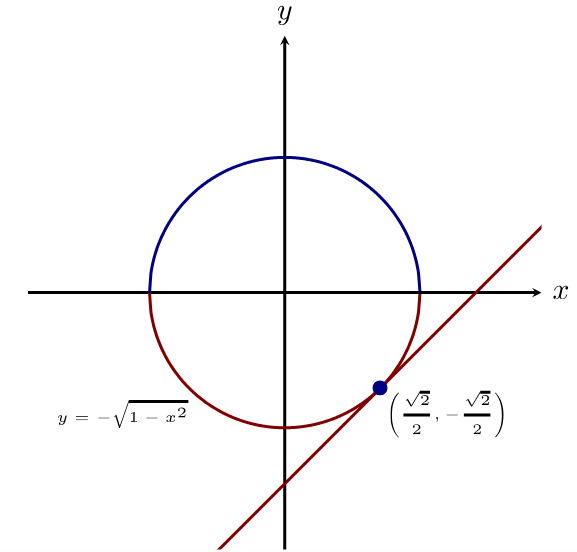
\includegraphics{1.png}
        \end{image}
On which of the following intervals is $f$ increasing?
\begin{selectAll}
\choice[correct]{$(-\infty,a)$}
\choice{$(-\infty,b)$}
\choice{$(a,b)$}
\choice{$(a,+\infty)$}
\choice[correct]{$(b,+\infty)$}
\end{selectAll}
\begin {explanation} The function $f$ is not increasing on the interval $(-\infty,b)$, because if we pick a pair of numbers from $(-\infty,b)$, say, $x_{1}=a$, and $x_{2}=0$,
then $x_{1}<x_{2}$, but  $f(x_{1})>f(x_{2})$.
\end {explanation}
\end{question}
\begin{question}
\author{Nela Lakos}
Which of the following famous functions are increasing on $\Bigl(0,\frac{\pi}{2}\Bigr)$?
\begin{selectAll}
\choice[correct]{$\sin{(x)}$}
\choice{$\sin{(2x)}$}
\choice{$\cos{(x)}$}
\choice[correct]{$\tan{(x)}$}
\choice{$\cot{(x)}$}
\choice[correct]{$f(x)=x^2$}
\choice{$g(x)=\dfrac{1}{x}$}
\end{selectAll}
\begin {explanation} The function $\cos{(x)}$ is not increasing on $I=\Bigl(0,\frac{\pi}{2}\Bigr)$, because 
if we take a pair of numbers in $I$, say,  
  $x_{1}=\frac{\pi}{6}$, and   $x_{2}=\frac{\pi}{3}$, then
   $x_{1}<x_{2}$,  but \\$f(x_{1})>f(x_{2})$,  since 
 $f(x_{1})=\cos{\Bigl(\frac{\pi}{6}\Bigr)}=\frac{\sqrt{3}}{2}$, and $f(x_{2})=\cos{}\Bigl(\frac{\pi}{3}\Bigr)=\frac{1}{2}$.
 \end{explanation}
\end{question}
Since the derivative gives us a formula for the slope of a tangent
line to a curve, we can gain information about a function purely from
the sign of the derivative.  In particular, we have the following theorem
\begin{theorem}
A function $f$ is \textbf{increasing} on any interval $I$ where $f'(x)>0$, for all $x$ in $I$.\\
A function $f$  is \textbf{decreasing} on any interval $I$ where $f'(x)<0$, for all $x$ in $I$.\\
 \end{theorem}


\begin{question}
  Below we have graphed $y=f'(x)$:
  \begin{image}
    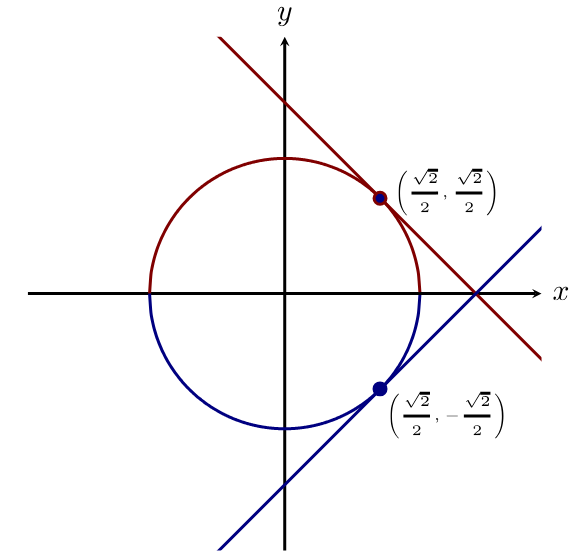
\includegraphics{2.png}
  \end{image}
  Is the function $f$ increasing or decreasing on
  the interval $-1<x<0$?
  \begin{prompt}
    \begin{multipleChoice}
      \choice[correct]{Increasing}
      \choice{Decreasing}
    \end{multipleChoice}
  \end{prompt}
  \begin{explanation} From the graph of  $f'$ we can see that $f'(x)>0$ for all $x$ in $(-1,0)$. Then, the Theorem above implies that the function $f$ is increasing on this interval.
      \end{explanation}
\end{question}

We call the derivative of the derivative the \dfn{second
  derivative}, the derivative of the second derivative (the derivative of the derivative of the derivative) the
\dfn{third derivative}, and so on. We have special notation for
higher derivatives, check it out:
\begin{description}
\item[First derivative:] $\ddx f(x) = f'(x) = f^{(1)}(x)$.
\item[Second derivative:] $\dd[~^2]{x^2} f(x) = f''(x) = f^{(2)}(x)$.
\item[Third derivative:] $\dd[~^3]{x^3} f(x) = f'''(x) = f^{(3)}(x)$.
\end{description}

We use the facts above in our next example.

\begin{example}
  Here we have unlabeled graphs of $f$, $f'$, and $f''$:
  \begin{image}
    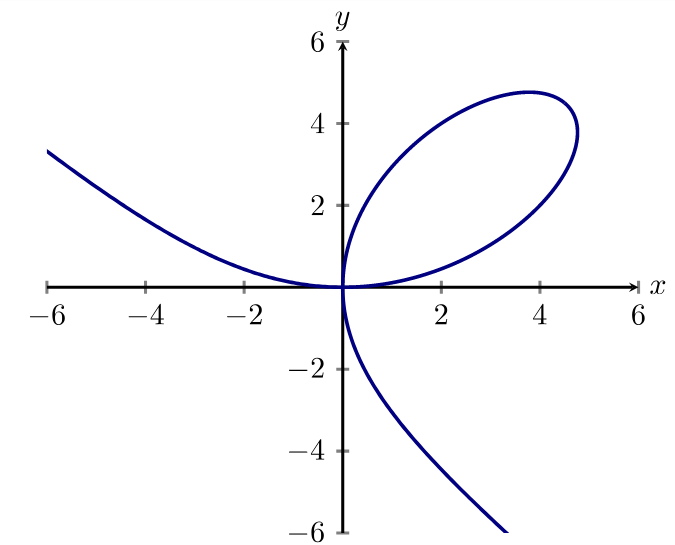
\includegraphics{3.png}
  \end{image}
  Identify each curve above as a graph of $f$, $f'$, or $f''$.
  \begin{explanation} 
    Here we see three curves, $A$, $B$, and $C$. Since $A$ is
    \wordChoice{\choice{positive} \choice{negative}
      \choice[correct]{increasing} \choice{decreasing}} when $B$ is
    positive and
    \wordChoice{\choice{positive}\choice{negative}\choice{increasing}\choice[correct]{decreasing}}
    when $B$ is negative, we see
    \[
    A'=B.
    \]
    Since $B$ is increasing when $C$ is
    \wordChoice{\choice[correct]{positive}\choice{negative}\choice{increasing}
      \choice{decreasing}} and decreasing when $C$ is
    \wordChoice{\choice{positive}\choice[correct]{negative}\choice{increasing}\choice{decreasing}}, we see
    \[
    B'=C.
    \]
    Hence $f=A$, $f'=B$, and $f''=C$.
  \end{explanation}
\end{example}




\begin{example}
    Here we have unlabeled graphs of $f$, $f'$, and $f''$:
\begin{image}
      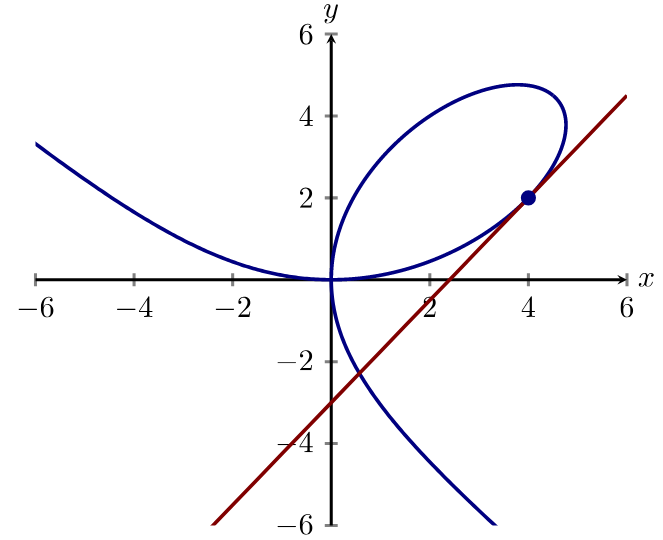
\includegraphics{4.png}
\end{image}
    Identify each curve above as a graph of $f$, $f'$, or $f''$.
      \begin{explanation} 
        Here we see three curves, $A$, $B$, and $C$. Since $B$ is
        \wordChoice{\choice{positive}\choice{negative}\choice[correct]{increasing}\choice{decreasing}} when $A$
        is positive and
        \wordChoice{\choice{positive}\choice{negative}\choice{increasing}\choice[correct]{decreasing}} when $A$
        is negative, we see
        \[
        B'=A.
        \]
        Since $A$ is increasing when $C$ is
        \wordChoice{\choice[correct]{positive}\choice{negative}\choice{increasing}\choice{decreasing}}
          and decreasing when $C$ is
          \wordChoice{\choice{positive}\choice[correct]{negative}\choice{increasing}\choice{decreasing}}, we
          see
        \[
        A'=C.
        \]
        Hence $f=\answer[given]{B}$, $f'=\answer[given]{A}$, and
        $f''=\answer[given]{C}$.
      \end{explanation}
\end{example}

\begin{example}
  Here we have unlabeled graphs of $f$, $f'$, and $f''$:
  \begin{image}
    \includegraphics{5.png}
  \end{image}
  Identify each curve above as a graph of $f$, $f'$, or $f''$.
  %One is of $f$, another is of $f'$ and a third is of $f''$.  Explain
  %what strategies you could use to identify which graph corresponds
    \begin{explanation} %%BADBAD Need Dropdown
    Here we see three curves, $A$, $B$, and $C$. Since $C$ is
    \wordChoice{\choice{positive}\choice{negative}\choice[correct]{increasing}\choice{decreasing}} when $B$ is
    positive and \wordChoice{\choice{positive}\choice{negative}\choice{increasing}\choice[correct]{decreasing}}
    when $B$ is negative, we see
    \[
    C'=B.
    \]
    Since $B$ is increasing when $A$ is
    \wordChoice{\choice[correct]{positive}\choice{negative}\choice{increasing}\choice{decreasing}} and
    decreasing when $A$ is
    \wordChoice{\choice{positive}\choice[correct]{negative}\choice{increasing}\choice{decreasing}}, we see
    \[
    B'=A.
    \]
    Hence $f=\answer[given]{C}$, $f'=\answer[given]{B}$, and
    $f''=\answer[given]{A}$.
  \end{explanation}
\end{example}


\end{document}
